\section{Thiết kế hệ thống}
\subsection{Kiến trúc tổng thể}

\begin{figure}[H]
    \centering
    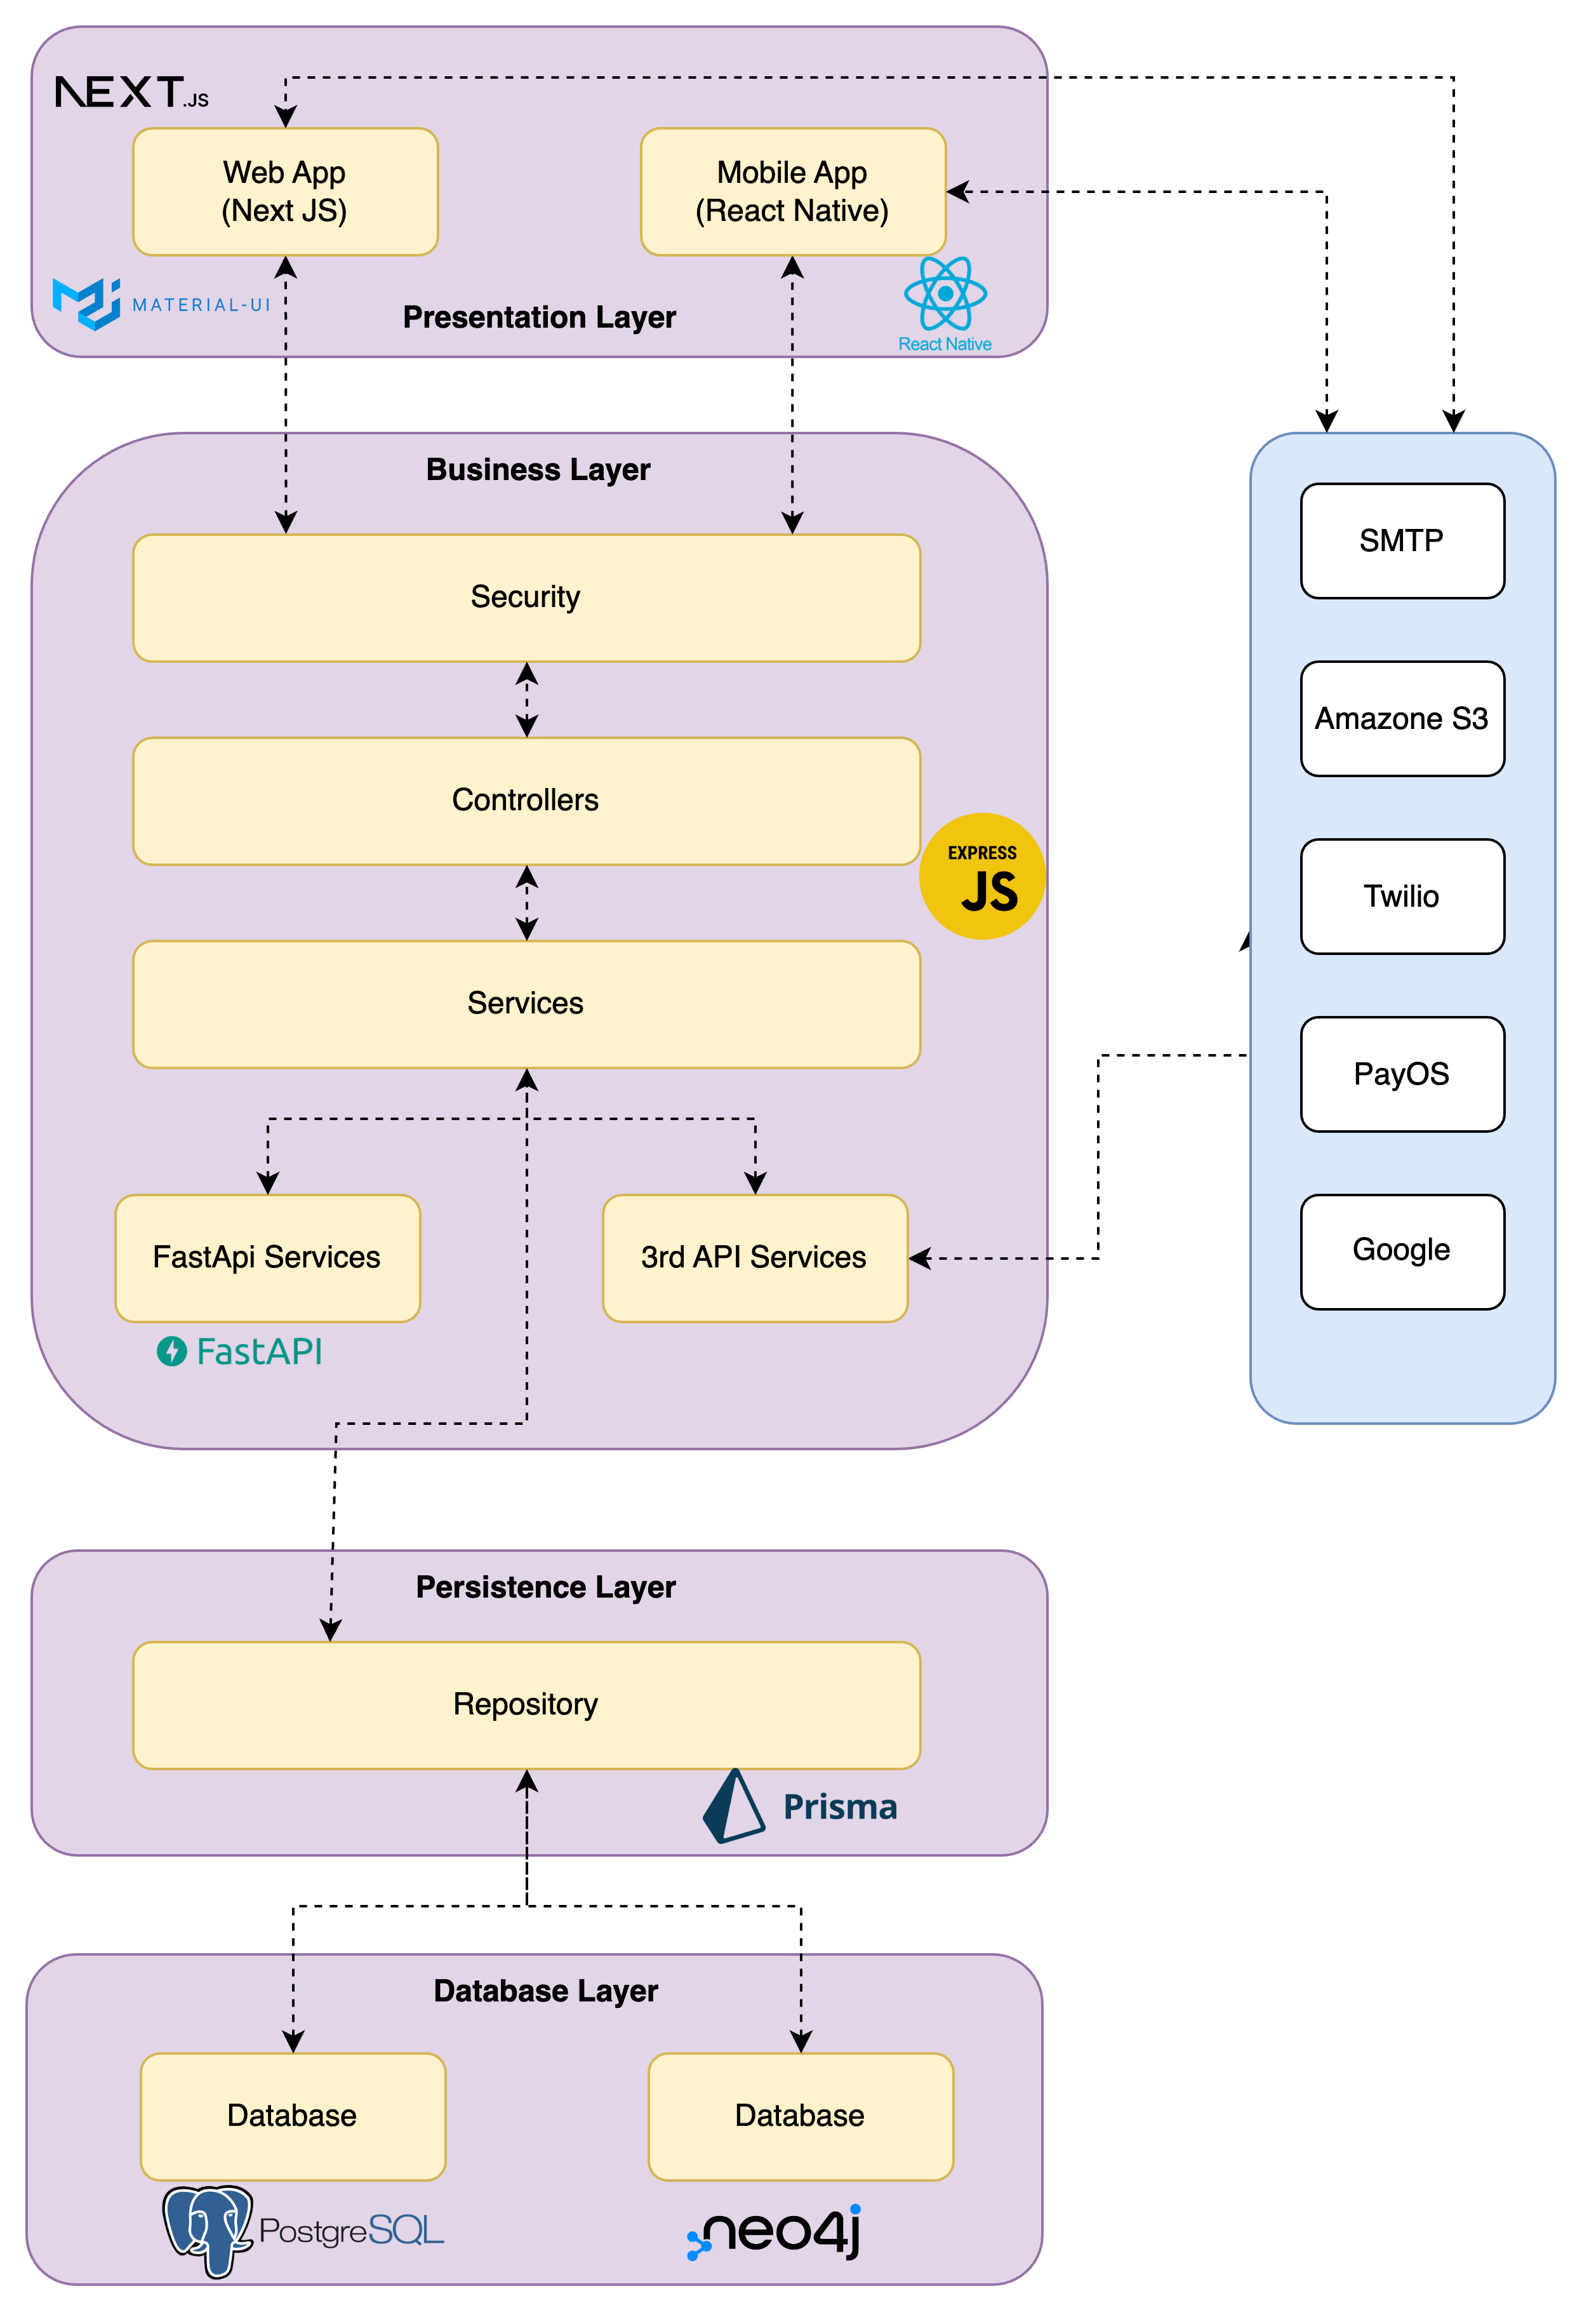
\includegraphics[width=13cm]{Images/architure_system.png}
    \vspace{1cm}
    \caption{Kiến trúc tổng quan của hệ thống}
    \label{fig:enter-label}
\end{figure}
\subsection{Thiết kế cơ sở dữ liệu}
\subsubsection{Thiết kế cơ sở dữ liệu ý niệm}
\begin{figure}[H]
            \centering
            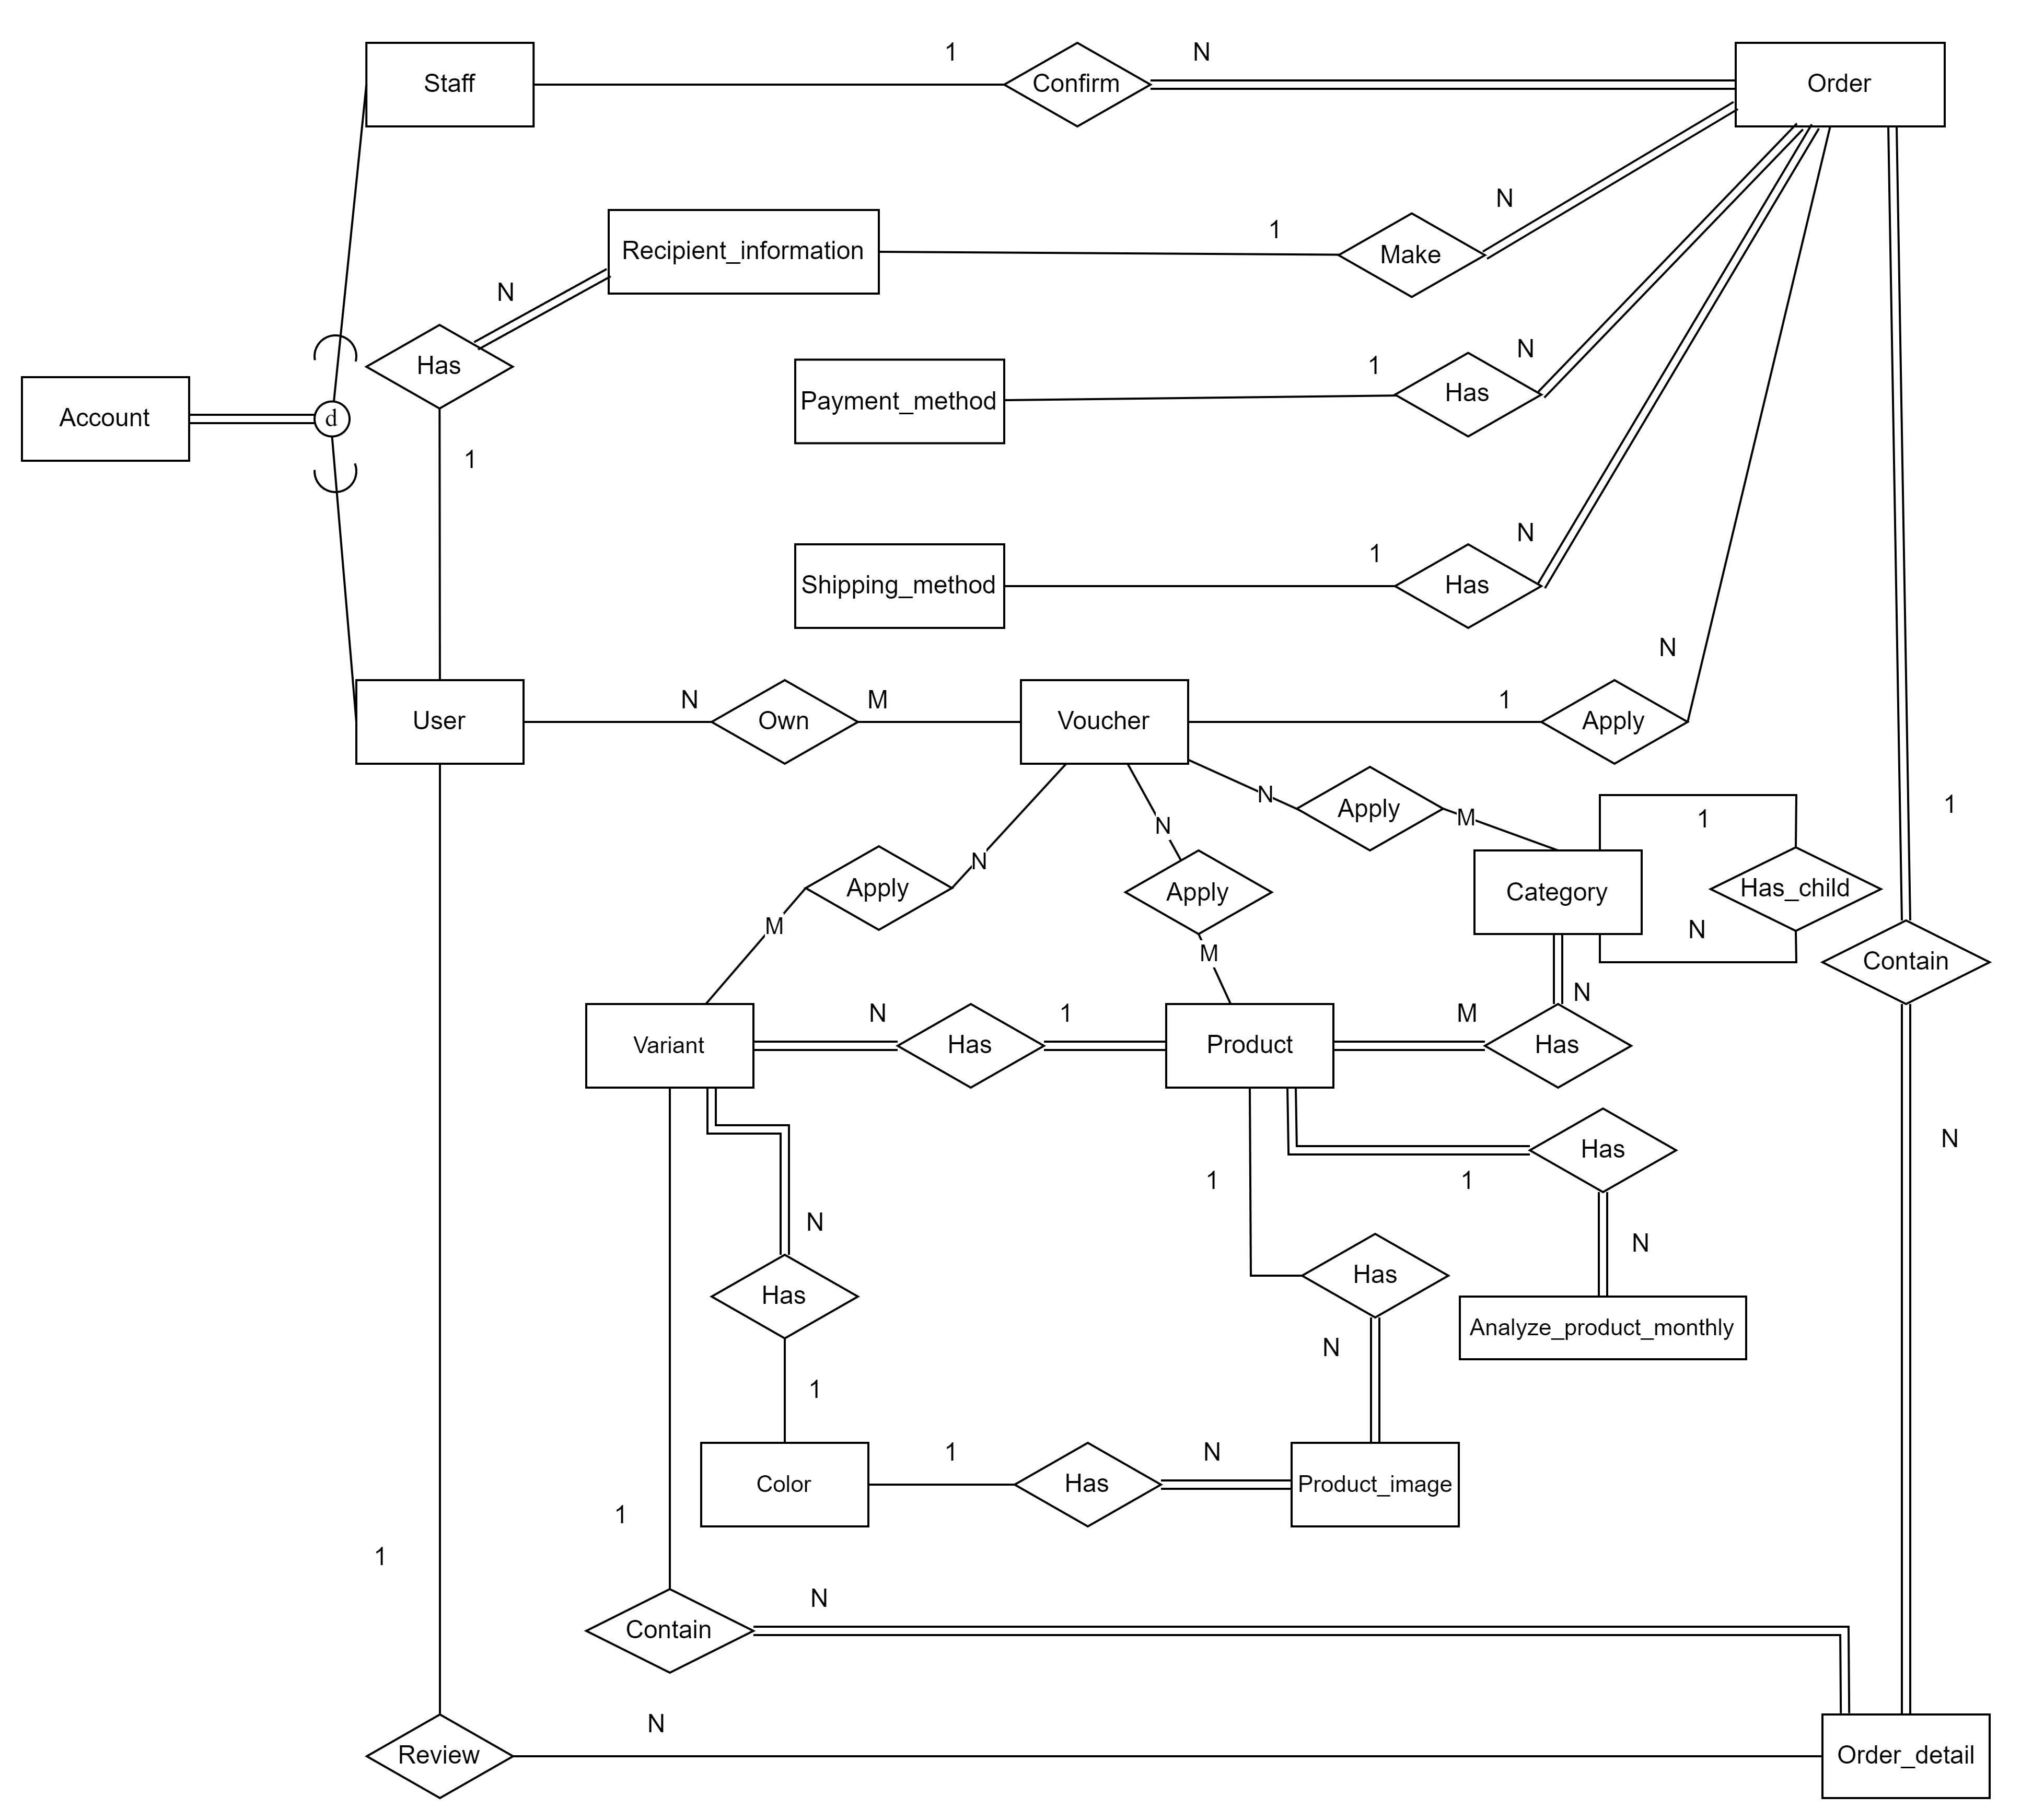
\includegraphics[width=15cm]{Images/ERD/ERD.png}
            \newline
            \newline
            \caption{Thiết kế tổng quan cơ sở dữ liệu ý niệm của cửa hàng thời trang}
            \label{fig:enter-label}
        \end{figure}
%     Các ràng buộc về quan hệ giữa các thực thể:\\
% \begin{itemize}
% \item Một user có thể có nhiều userInfo
% \item Một user có thể sở hữu nhiều voucher
% \item Một user chỉ có một cart
% \item Một user có thể viết nhiều bài review 
% \item Một voucher có thể được sở hữu bởi nhiều user
% \item Một staff có thể xác nhận nhiều đơn hàng
% \item Một user info có thể tạo nhều đơn hàng
% \item Một order chỉ có một phương thức thanh toán
% \item Một order chỉ có một phương thức vận chuyển
% \item Một đơn hàng có thể chứa nhiều đơn hàng chi tiết
% \item 
% \item 
% \item 
% \item 
% \item 
% \end{itemize}
\begin{figure}[H]
            \centering
            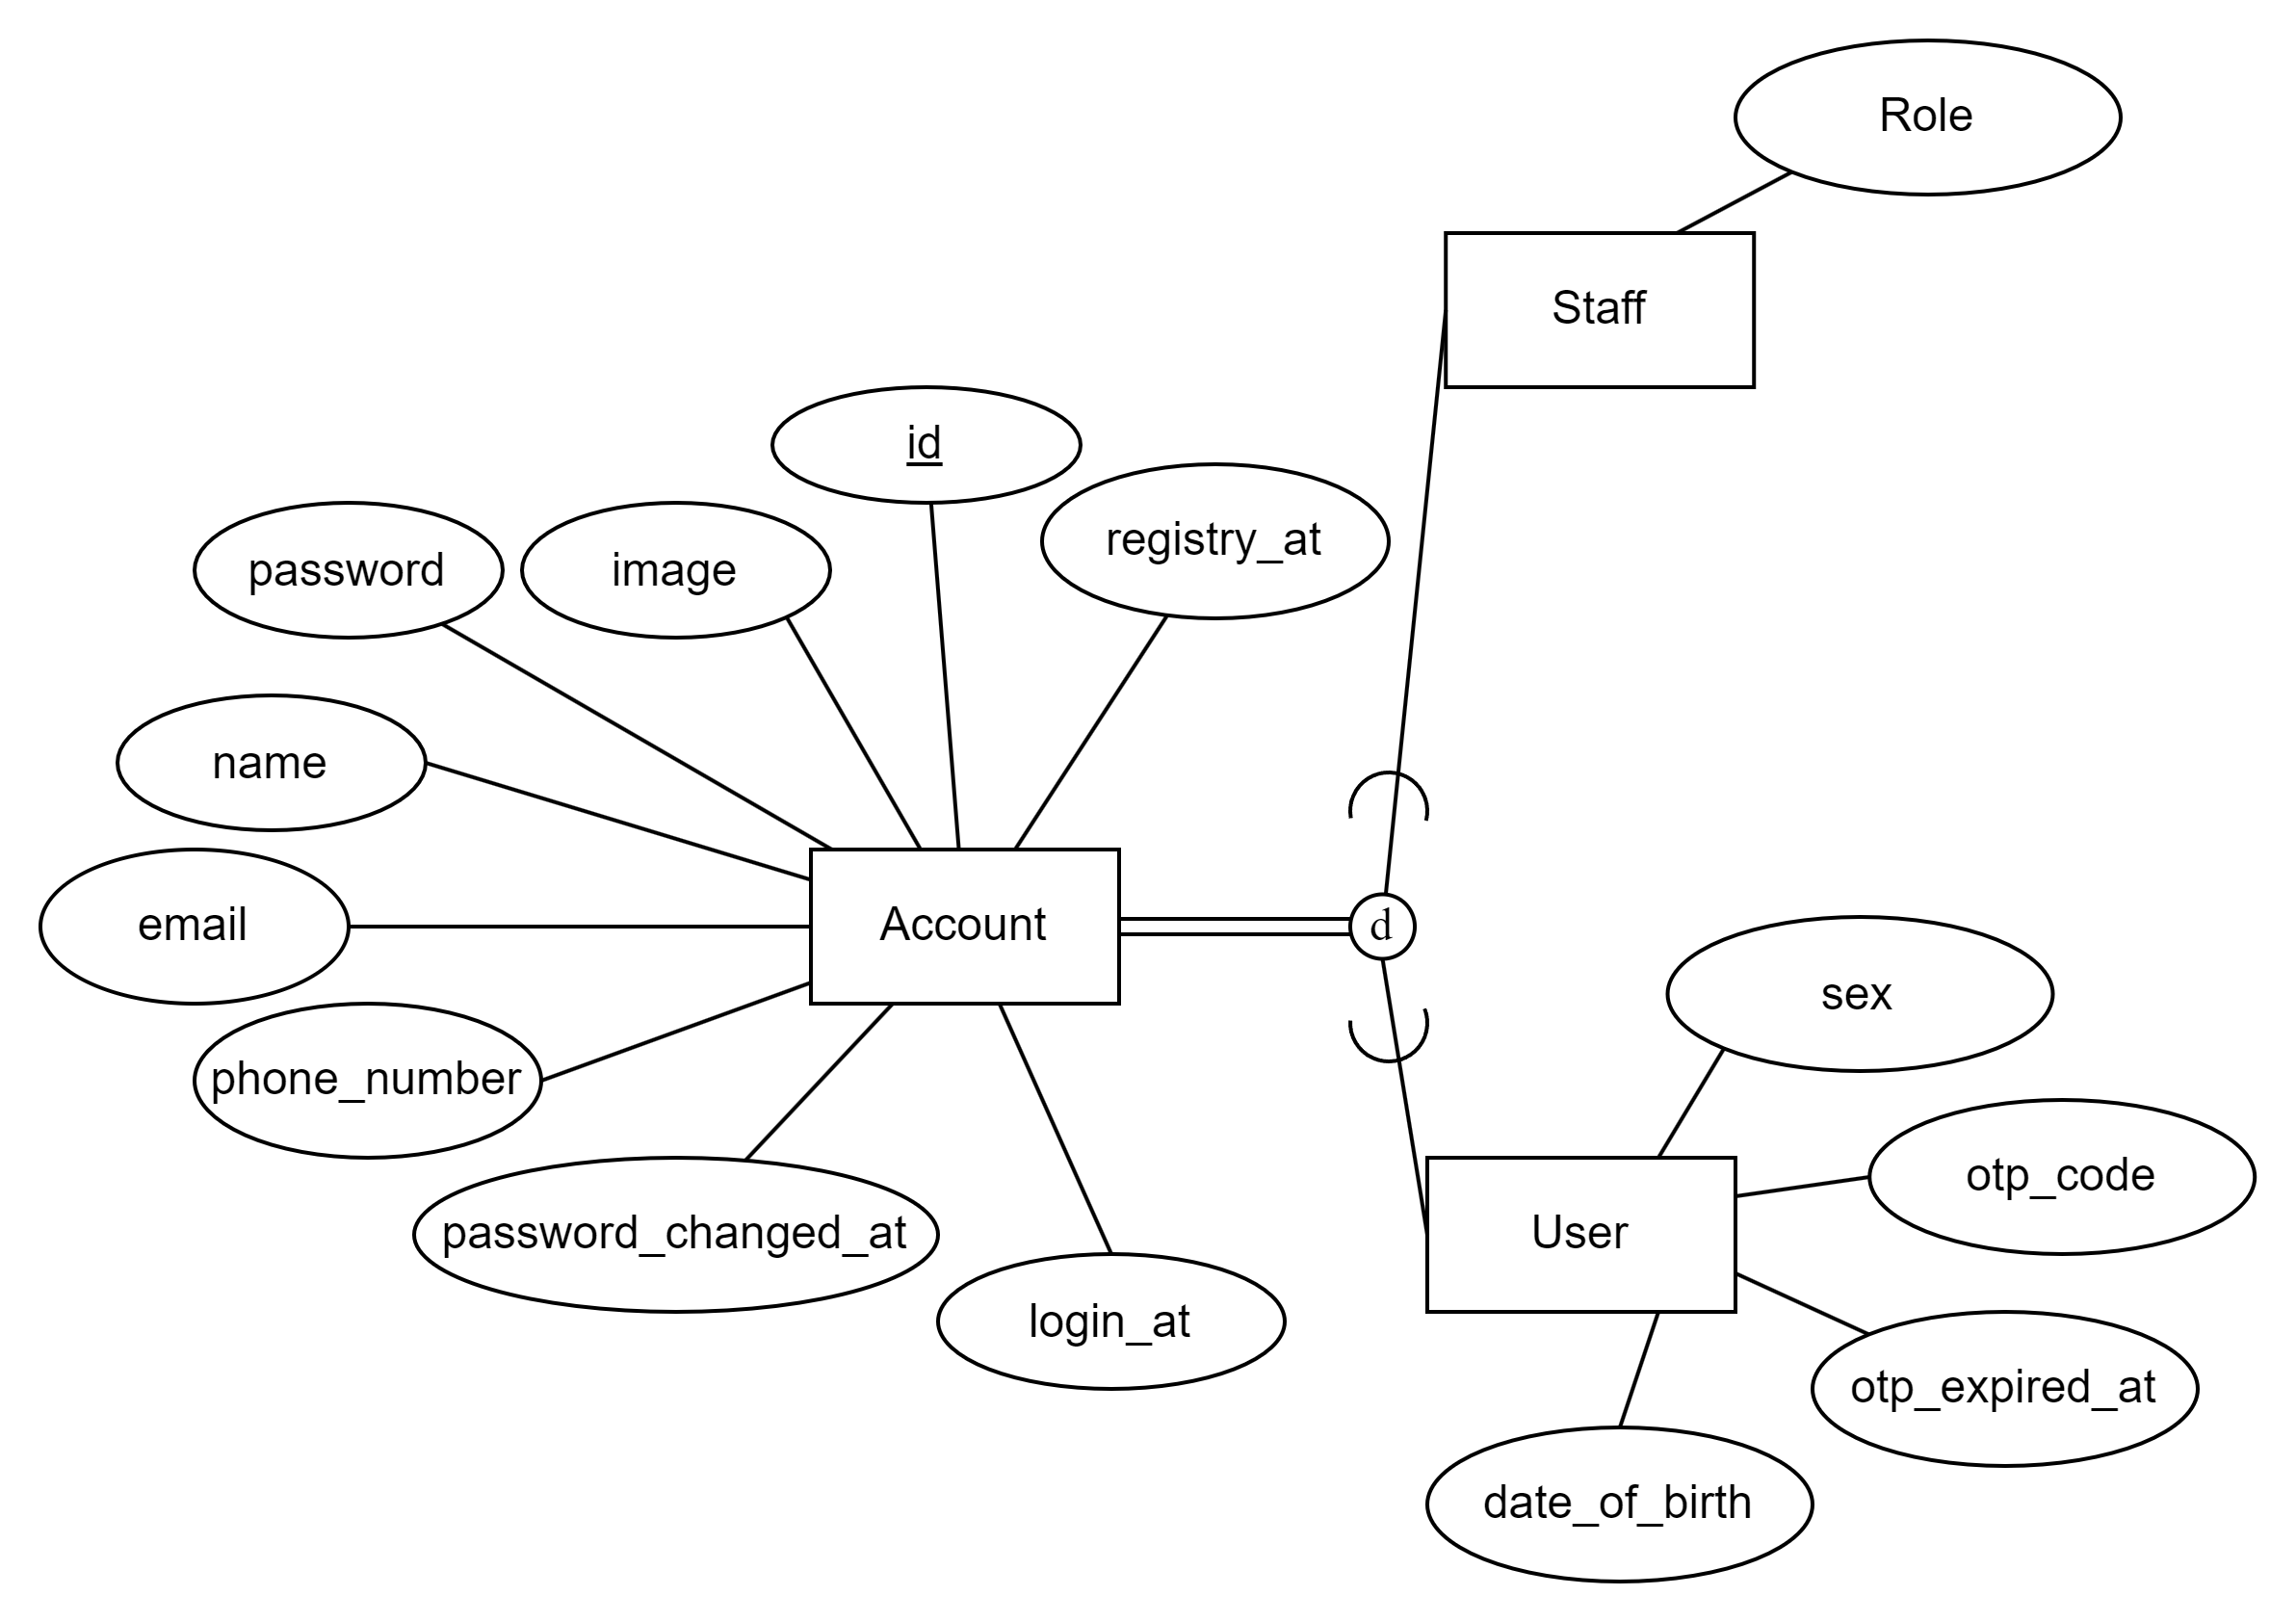
\includegraphics[width=15cm]{Images/ERD/account.png}
            \newline
            \caption{Chi tiết thiết kế của thực thể Account}
            \label{fig:enter-label}
        \end{figure}
        
Các thuộc tính của thực thể Account:
\begin{itemize}
    \item id: Khóa chính, dùng để định danh tài khoản
    \item image: Ảnh đại diện của tài khoản 
\item name: Tên đầy đủ của tài khoản 
\item email: Email của tài khoản 
\item phone number: Số điện thoại của tài khoản
\item password: Mật khẩu của tài khoản
\item password change at: Thời gian gần nhất mà mật khẩu được thay đổi
\item login at: Thời gian của lần đăng nhập gần nhất
\item registry at: Thời gian mà tài khoản được tạo
\end{itemize}

\begin{figure}[H]
            \centering
            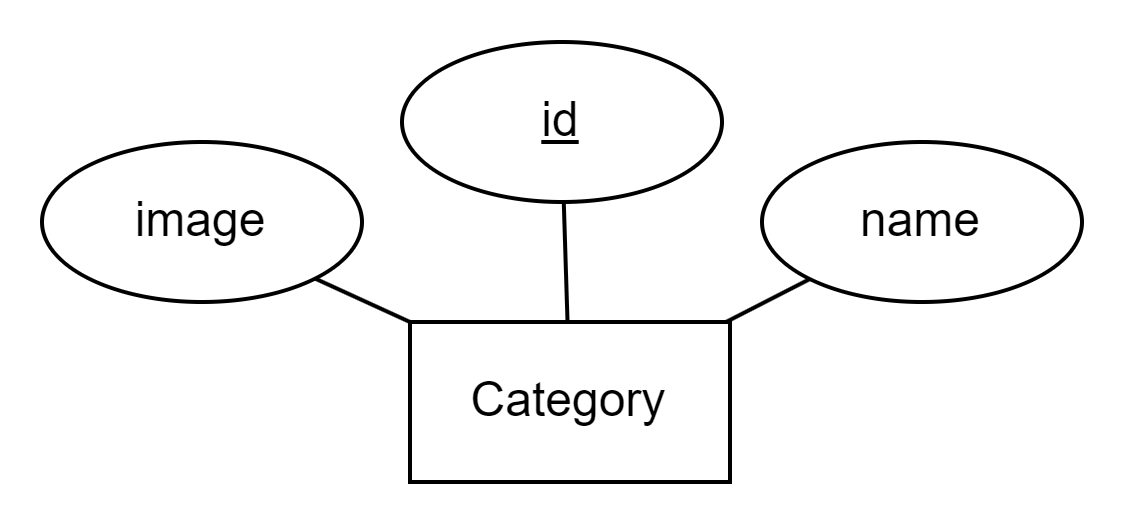
\includegraphics[width=11cm]{Images/ERD/category.png}
            \newline
            \caption{Chi tiết thiết kế của thực thể Category}
            \label{fig:enter-label}
        \end{figure}
        
Các thuộc tính của thực thể Category:
\begin{itemize}
    \item id: Khóa chính, dùng để định danh thể loại/danh mục
    \item name: Tên của thể loại/danh mục
    \item image: Ảnh của thể loại/danh mục
\end{itemize}
% \begin{figure}[H]
%             \centering
%             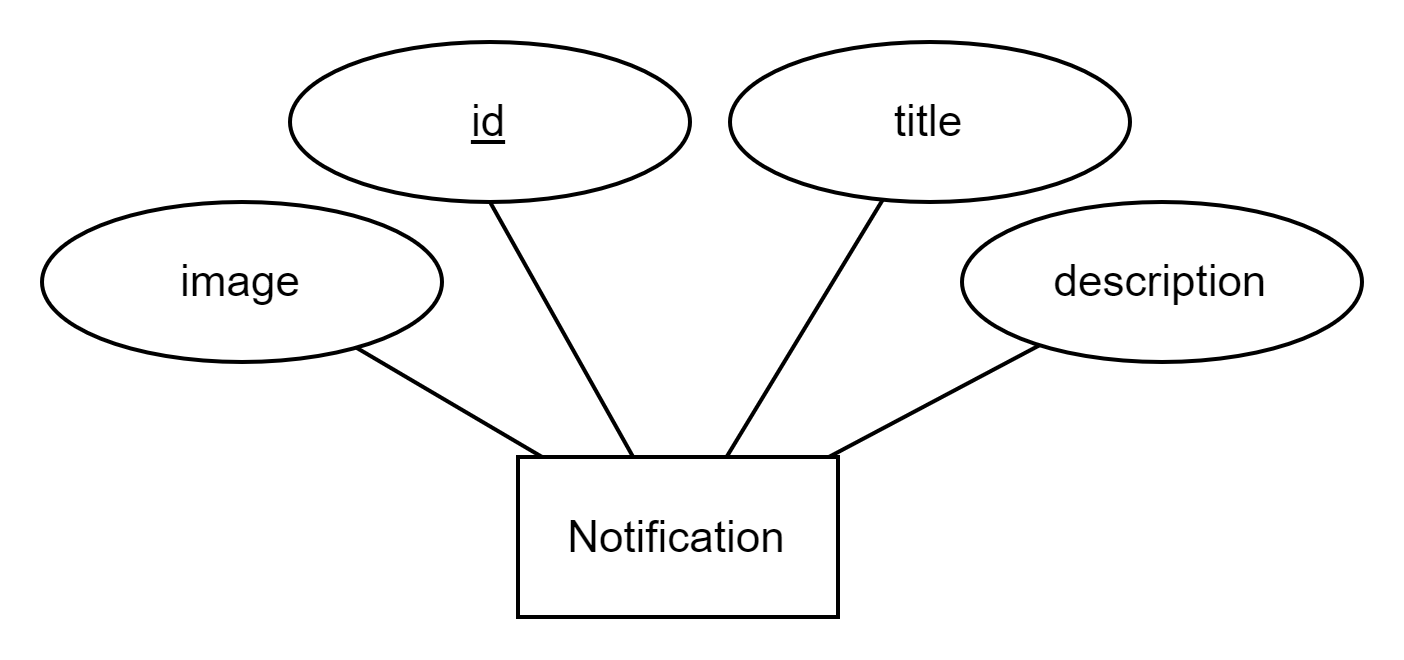
\includegraphics[width=15cm]{Images/ERD/notification.png}
%             \newline
%             \caption{Chi tiết thiết kế của thực thể Notification}
%             \label{fig:enter-label}
%         \end{figure}
% Các thuộc tính của thực thể Notification:
% \begin{itemize}
%     \item id: Khóa chính, dùng để định danh cho thông báo
%     \item title: Tiêu đề của thông báo
%     \item description: Mô tả chi tiết của thông báo
%     \item image: Hình ảnh hiển thị cho thông báo
% \end{itemize}
% \begin{figure}[H]
%             \centering
%             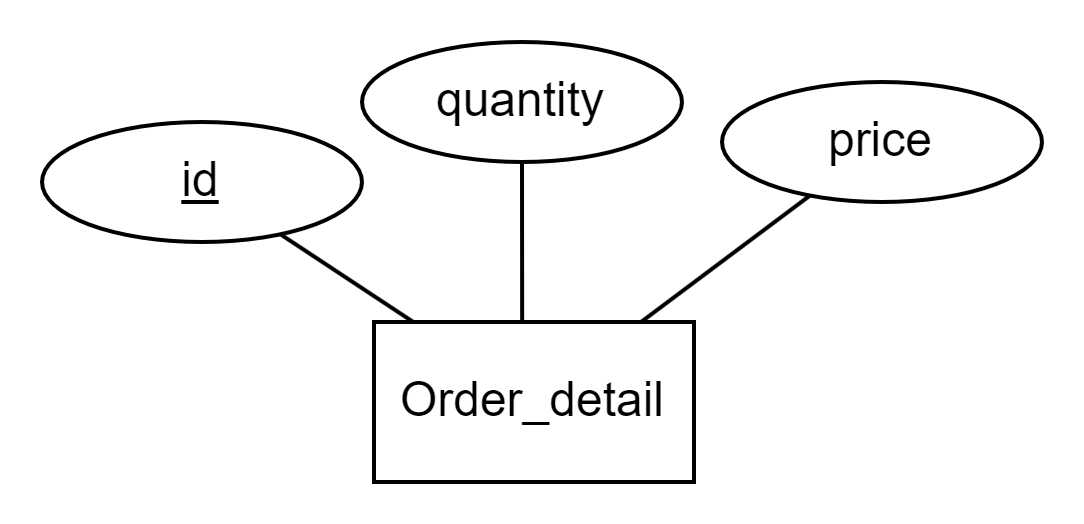
\includegraphics[width=11cm]{Images/ERD/order_detail.png}
%             \newline
%             \caption{Chi tiết thiết kế của thực thể Order Detail}
%             \label{fig:enter-label}
%         \end{figure}
% Các thuộc tính của thực thể Order Detail:
% \begin{itemize}
%     \item id: Khóa chính, dùng để định danh cho đơn hàng chi tiết
%     \item quantity: Số lượng sản phẩm trong đơn hàng chi tiết
% \end{itemize}
\begin{figure}[H]
            \centering
            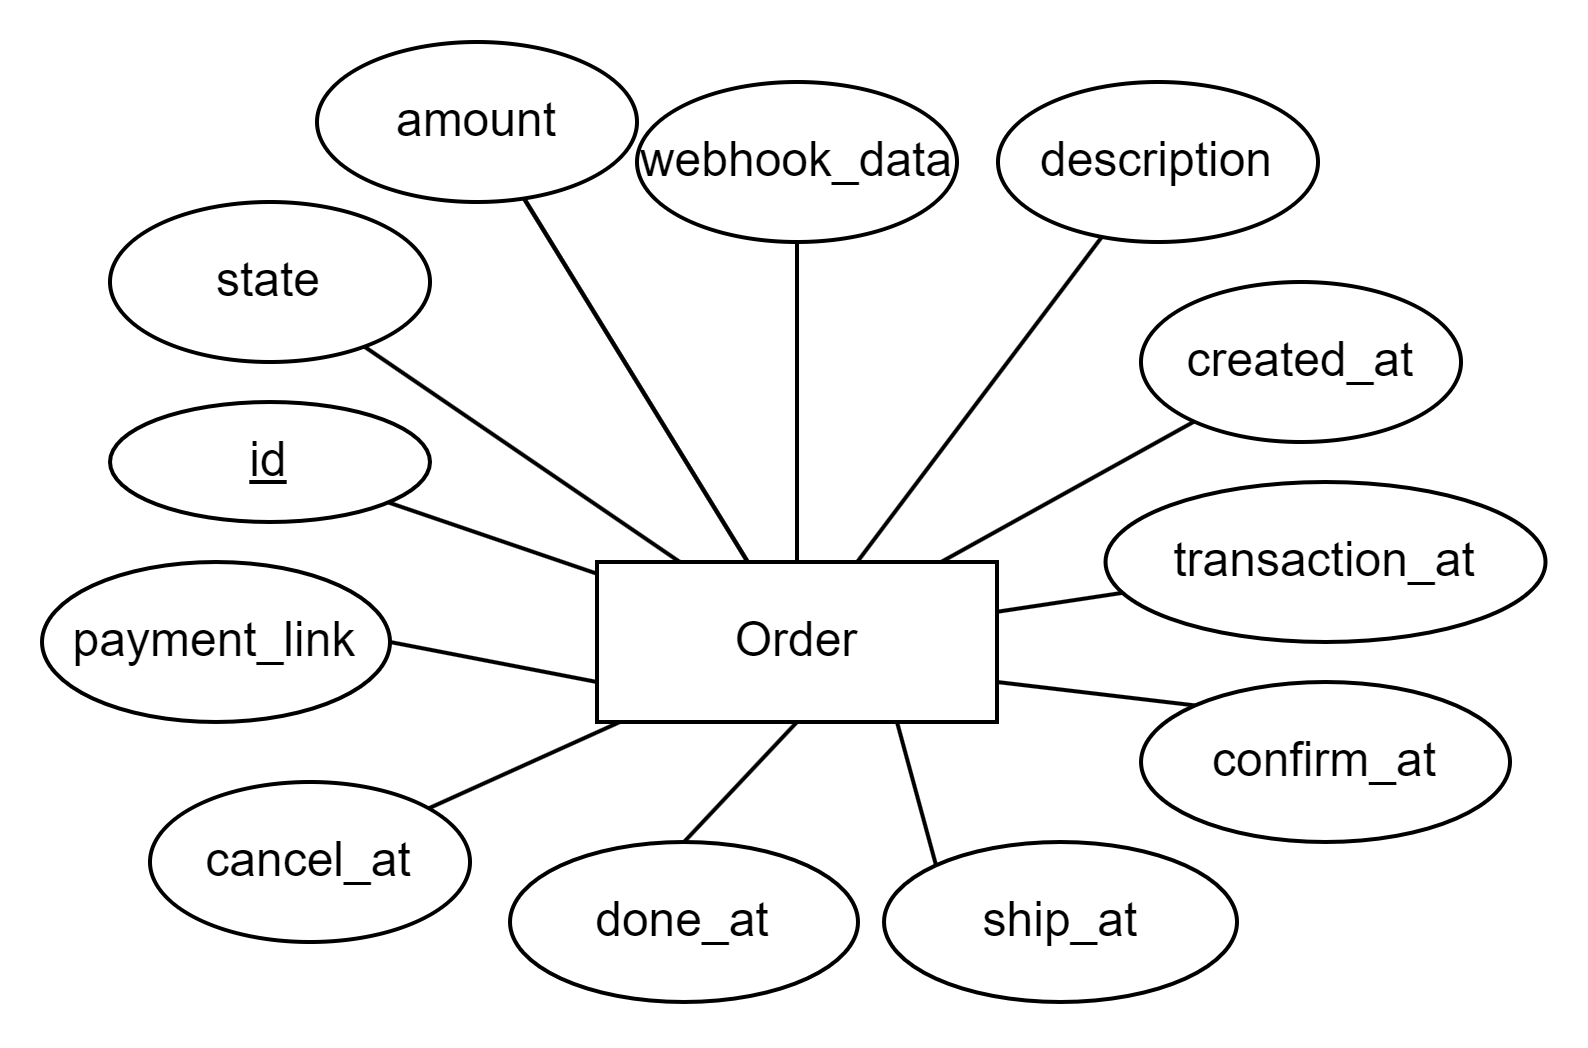
\includegraphics[width=15cm]{Images/ERD/order.png}
            \newline
            \caption{Chi tiết thiết kế của thực thể Order}
            \label{fig:enter-label}
        \end{figure}

\newpage       
Các thuộc tính của thực thể Order:
\begin{itemize}
    \item id: Khóa chính, dùng để định danh cho mỗi đơn hàng
    \item state: Trạng thái của đơn hàng
    \item amount: Tổng tiền của đơn hàng
    \item description: Mô tả chi tiết của đơn hàng
    \item create at: Thời gian đơn hàng được tạo
    \item transaction when: Thời điểm thanh toán
    \item webhook data: Thông tin thanh toán
    \item confirm at: Thời điểm đơn hàng được chấp thuận từ staff
    \item ship at: Thời điểm đơn hàng tiến hành vận chuyển
    \item done at: Thời điểm đơn hàng hoàn thành
    \item cancel at: Thời điểm đơn hàng bị hủy
    \item payment link: Đường dẫn thanh toán điện tử
\end{itemize}
\begin{figure}[H]
            \centering
            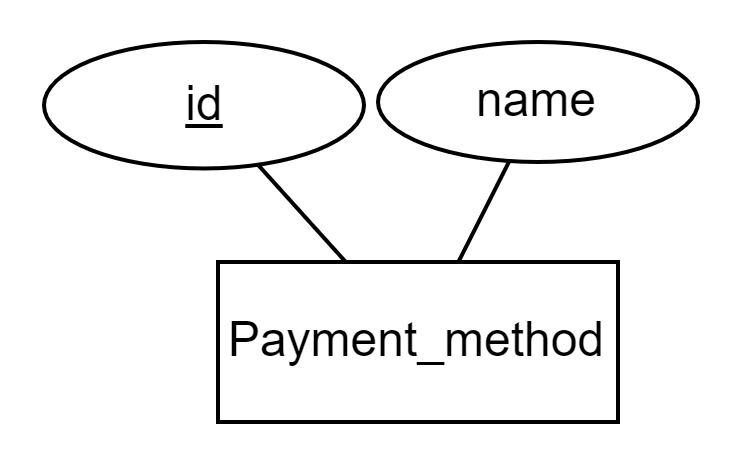
\includegraphics[width=10cm]{Images/ERD/payment_method.png}
            \newline
            \caption{Chi tiết thiết kế của thực thể Payment Method}
            \label{fig:enter-label}
        \end{figure}
        
Các thuộc tính của thực thể Payment Method:
\begin{itemize}
    \item id: Khóa chính, dùng để định danh cho mỗi phương thức thanh toán
    \item name: Tên của phương thức thanh toán
\end{itemize}
\begin{figure}[H]
            \centering
            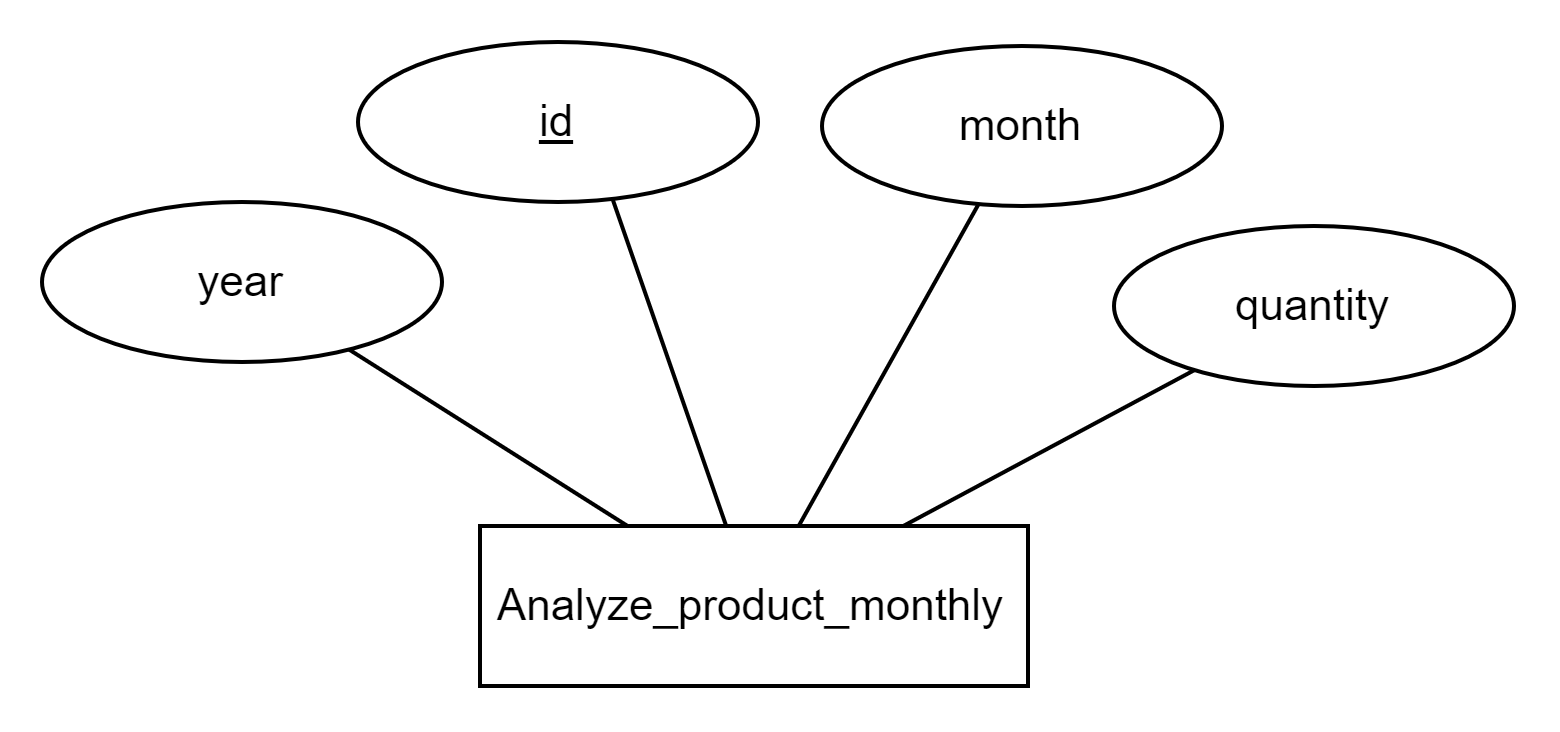
\includegraphics[width=15cm]{Images/ERD/product_bought.png}
            \newline
            \caption{Chi tiết thiết kế của thực thể Analyze product monthly}
            \label{fig:enter-label}
        \end{figure}
Các thuộc tính của thực thể Analyze product monthly:
\begin{itemize}
    \item id: Khóa chính, dùng để định danh cho mỗi sản phẩm bán chạy
    \item month: Sản phẩm bán chạy trong tháng n
    \item year: Sản phẩm bán chạy trong năm m
    \item quantity: Số lượng sản phẩm đó được bán ra trong tháng-năm đó
\end{itemize}
\begin{figure}[H]
            \centering
            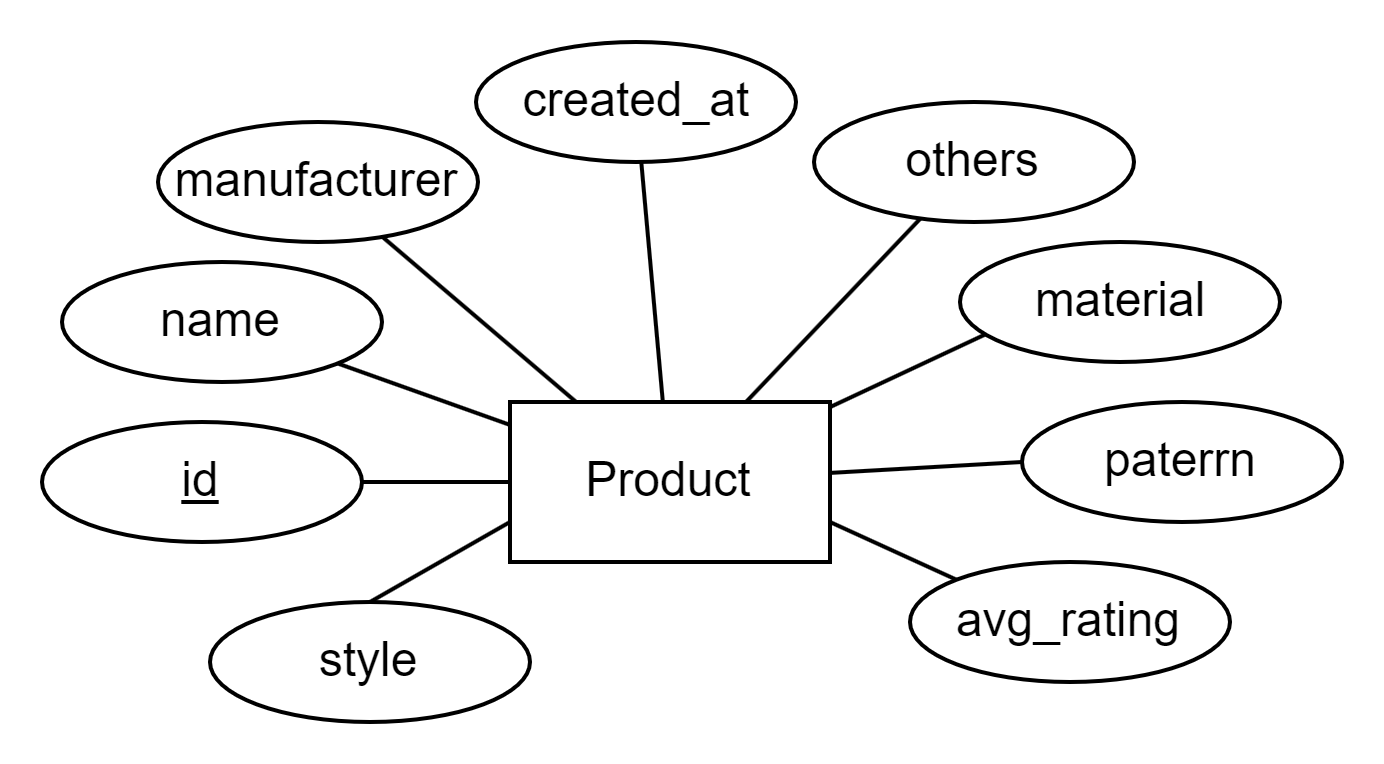
\includegraphics[width=15cm]{Images/ERD/product.png}
            \newline
            \caption{Chi tiết thiết kế của thực thể Product}
            \label{fig:enter-label}
        \end{figure}

\newpage
Các thuộc tính của thực thể Product:
\begin{itemize}
    \item id: Khóa chính, dùng để định danh cho mỗi sản phẩm
    \item name: Tên sản phẩm
    \item manufacturer: Tên nhà sản xuất cho sản phẩm đó
    \item create at: Ngày sản phẩm được thêm vào hệ thống
    \item others: Mô tả cho sản phẩm
    \item material: Chất liệu của sản phẩm
    \item pattern: Họa tiết sản phẩm
    \item style: Phong cách của sản phẩm
    \item avg rating: Đánh giá trung bình của sản phẩm
\end{itemize}
% \begin{figure}[H]
%             \centering
%             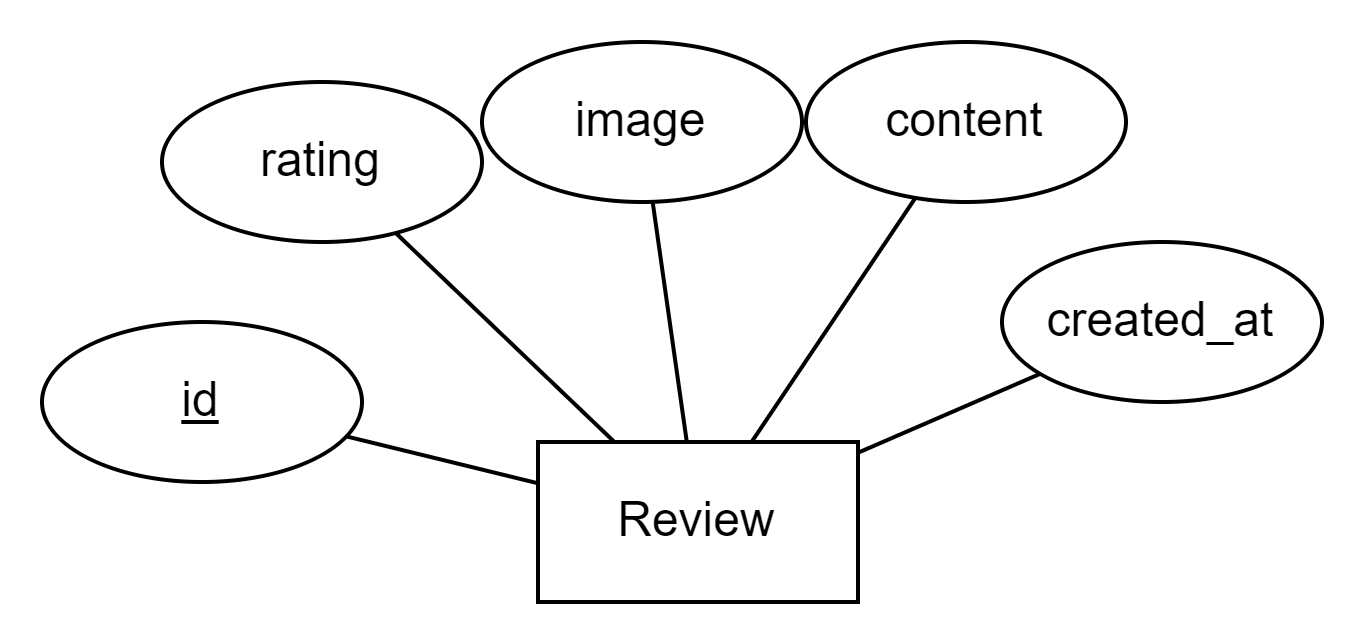
\includegraphics[width=15cm]{Images/ERD/review.png}
%             \newline
%             \caption{Chi tiết thiết kế của thực thể Review}
%             \label{fig:enter-label}
%         \end{figure}
% Các thuộc tính của thực thể Review:
% \begin{itemize}
%     \item id: Khóa chính, dùng để định danh cho mỗi bài đánh giá sản phẩm
%     \item rating: Số sao danh của bài viết đánh giá cho sản phẩm
%     \item content: Nội dung của bài đánh giá
%     \item create at: Ngày mà bài đánh giá được người dùng tạo trên hệ thống
%     \item image: Hình ảnh của người dùng tải lên cho bài đánh giá
% \end{itemize}
\begin{figure}[H]
            \centering
            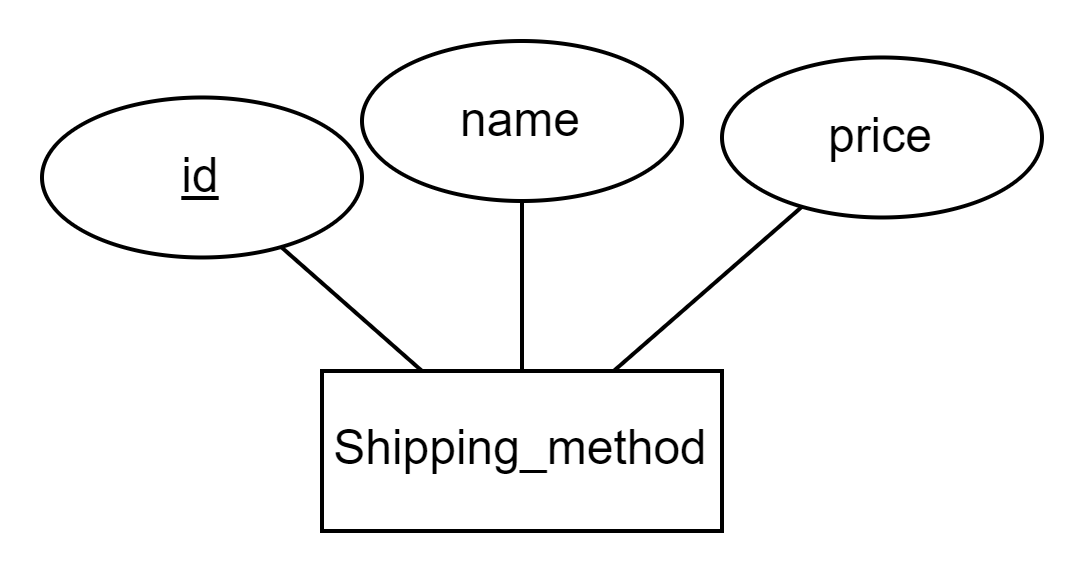
\includegraphics[width=13cm]{Images/ERD/shipping_method.png}
            \newline
            \caption{Chi tiết thiết kế của thực thể Shipping Method}
            \label{fig:enter-label}
        \end{figure}
Các thuộc tính của thực thể Shipping Method:
\begin{itemize}
    \item id: Khóa chính, dùng để định danh cho mỗi phương thức vận chuyển
    \item name: Tên phương thức vận chuyển
    \item price: Giá vận chuyển của phương thức vận chuyển đó
\end{itemize}
\begin{figure}[H]
            \centering
            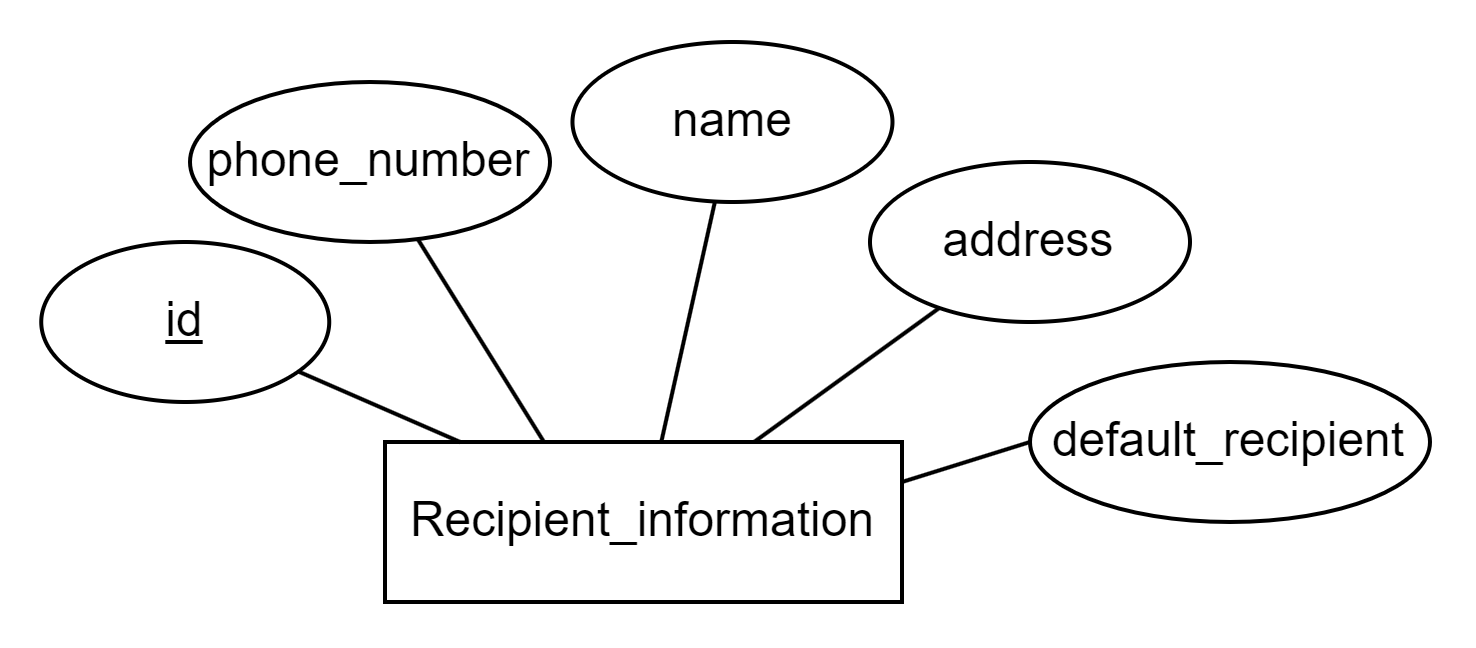
\includegraphics[width=15cm]{Images/ERD/user_info.png}
            \newline
            \caption{Chi tiết thiết kế của thực thể Recipient information}
            \label{fig:enter-label}
        \end{figure}

Các thuộc tính của thực thể Recipient information:
\begin{itemize}
    \item id: Khóa chính, dùng để định danh cho mỗi Thông tin người dùng
    \item address: Địa chỉ nhận hàng của người dùng
    \item name: Tên của người nhận hàng
    \item phone number: Số điện thoại của người nhận hàng
    \item default recipient: Thiết lập thông tin nhận hàng mặc định
\end{itemize}
\begin{figure}[H]
            \centering
            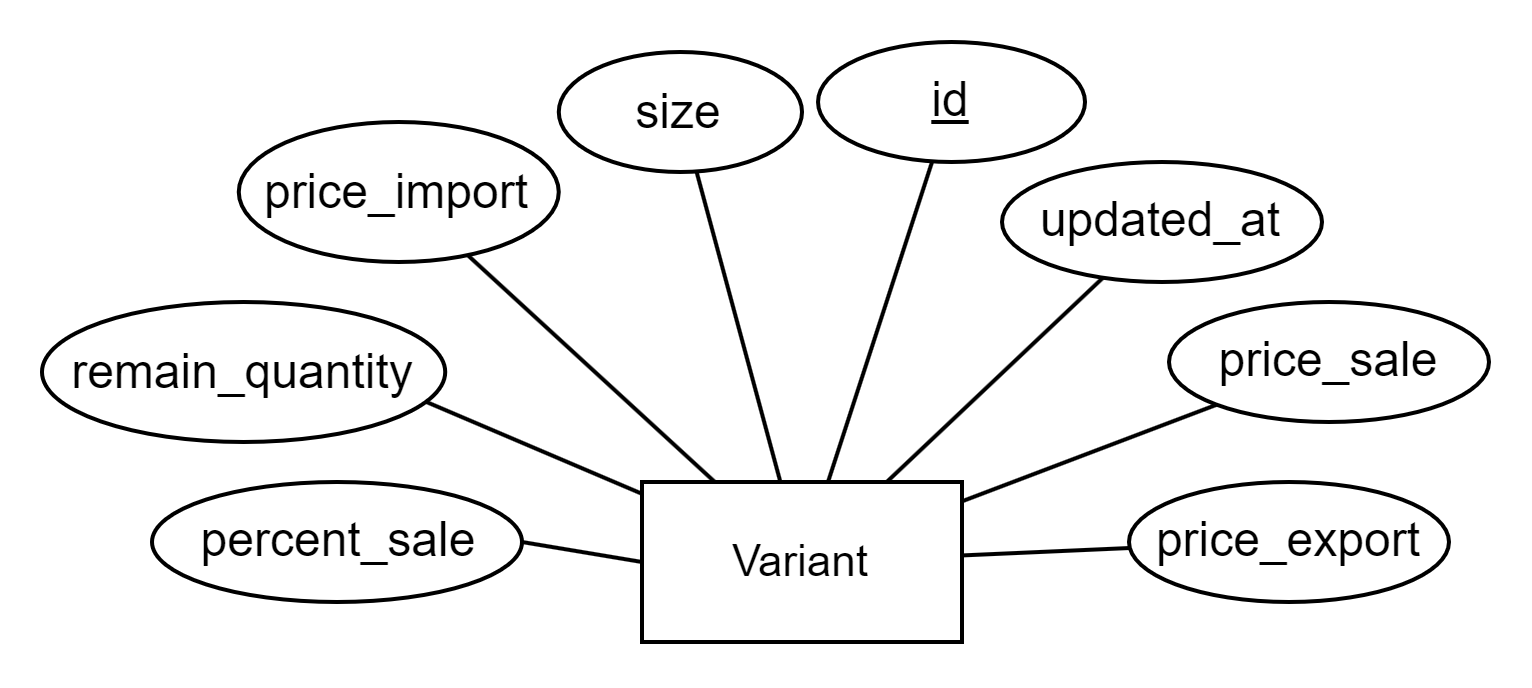
\includegraphics[width=15cm]{Images/ERD/variant.png}
            \newline
            \caption{Chi tiết thiết kế của thực thể Variant}
            \label{fig:enter-label}
        \end{figure}

\newpage
Các thuộc tính của thực thể Variant:
\begin{itemize}
\item id: Khóa chính, dùng để định danh cho mỗi biến sản phẩm
\item size: Kích cỡ của sản phẩm
\item price import: Giá nhập vào của sản phẩm
\item price sale: Giá của sản phẩm sau khi được giảm giá
\item remain quantity: Số lượng còn lại của sản phẩm
\item price export: Giá bán của sản phẩm
\item update at: Thời gian gần nhất sản phẩm được cập nhật
\item percent sale: Phần trăm giảm giá của sản phẩm
\end{itemize}
\begin{figure}[H]
            \centering
            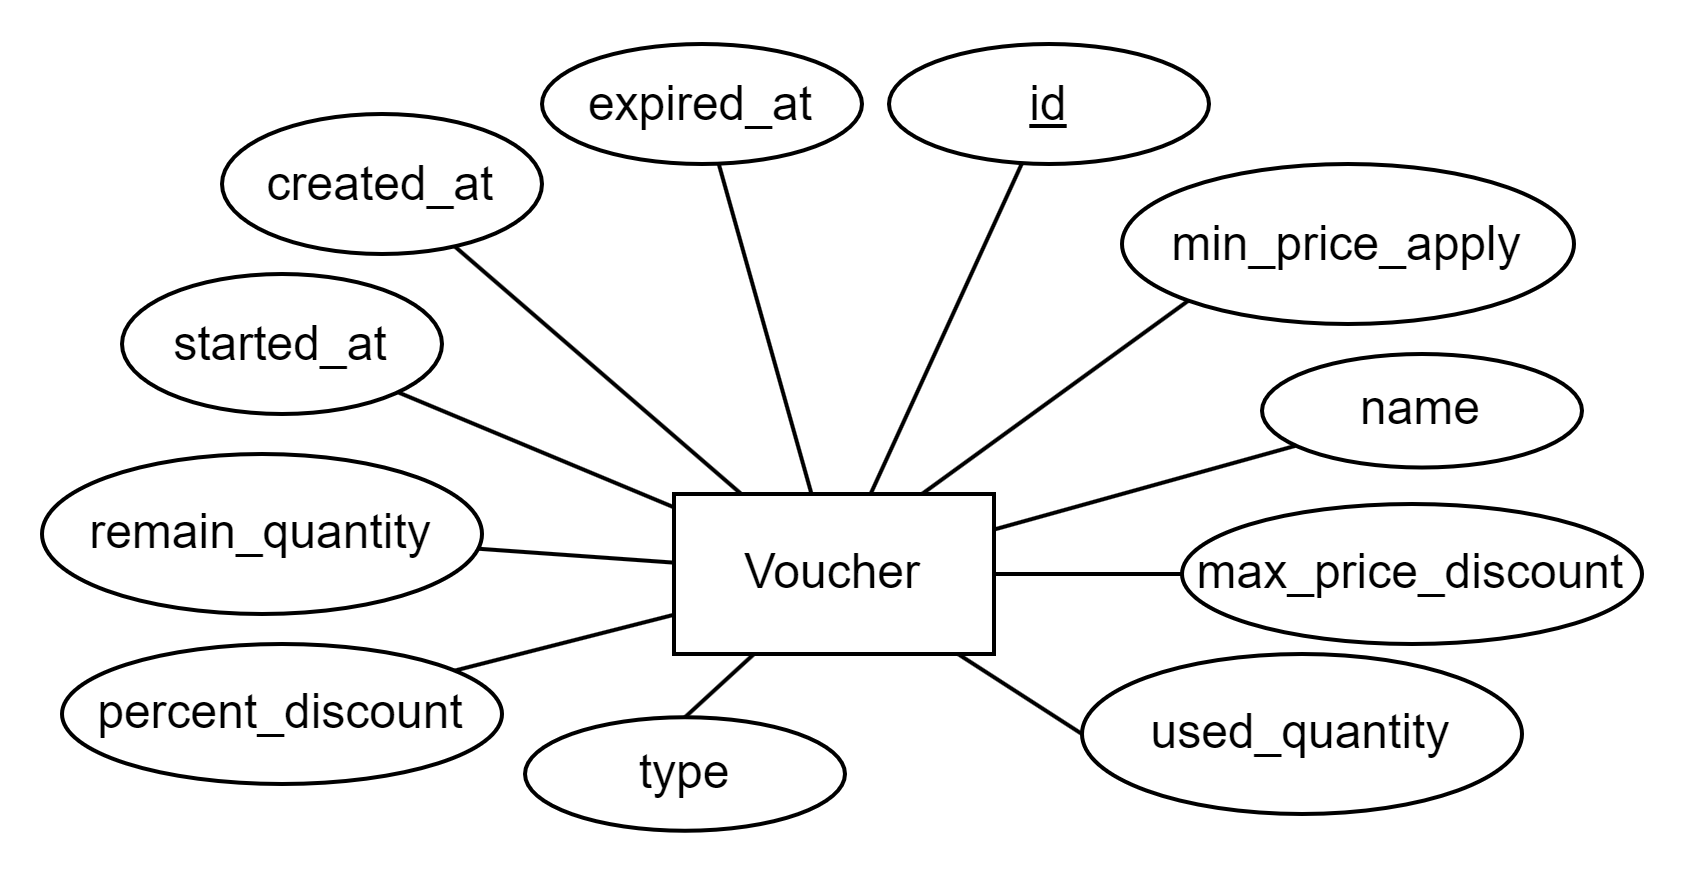
\includegraphics[width=15cm]{Images/ERD/voucher.png}
            \newline
            \caption{Chi tiết thiết kế của thực thể Voucher}
            \label{fig:enter-label}
\end{figure}
Các thuộc tính của thực thể Voucher:
\begin{itemize}
\item id: Khóa chính, dùng để định danh cho mỗi mã giảm giá
\item name: Tên của mã giảm giá
\item expire at: Ngày hết hạn của mã giảm giá
\item create at: Ngày tạo mã giảm giá
\item started at: Ngày bắt đầu có hiệu lực của mã giảm giá
\item remain quantity: Số lượng còn lại của mã giảm giá
\item percent discount: Phần trăm giảm giá của voucher
\item min price apply: Số tiền tối thiểu để có thể áp dụng voucher
\item max price discount: Số tiền tối đa có thể được giảm từ voucher 
\item type: Loại hình voucher
\item used quantity: số lượng voucher đã được sử dụng
\end{itemize}

\begin{figure}[H]
            \centering
            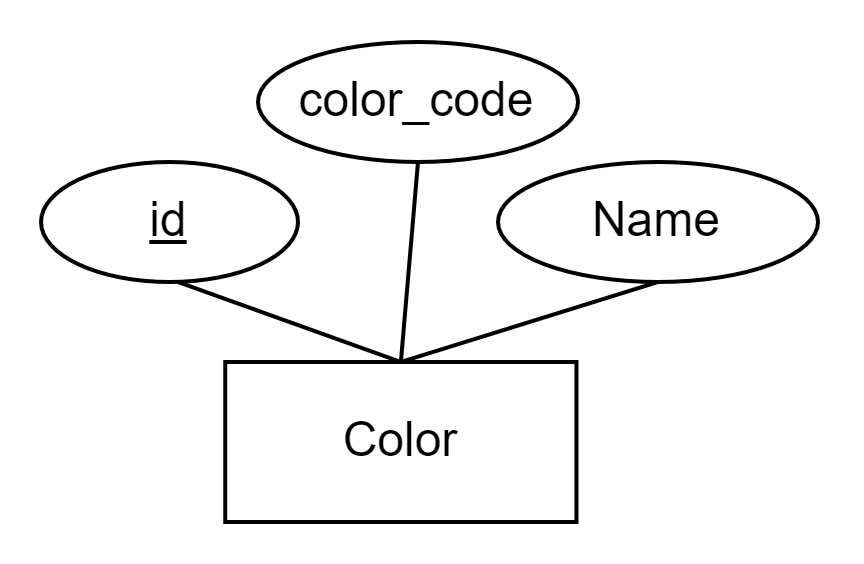
\includegraphics[width=11cm]{Images/ERD/color.png}
            \newline
            \caption{Chi tiết thiết kế của thực thể Color}
            \label{fig:enter-label}
\end{figure}
Các thuộc tính của thực thể Color:
\begin{itemize}
\item id: Khóa chính, dùng để định danh cho mỗi màu sắc
\item name: Tên của màu
\item color code: Mãu màu dạng HEX
\end{itemize}
\newpage
\begin{figure}[H]
            \centering
            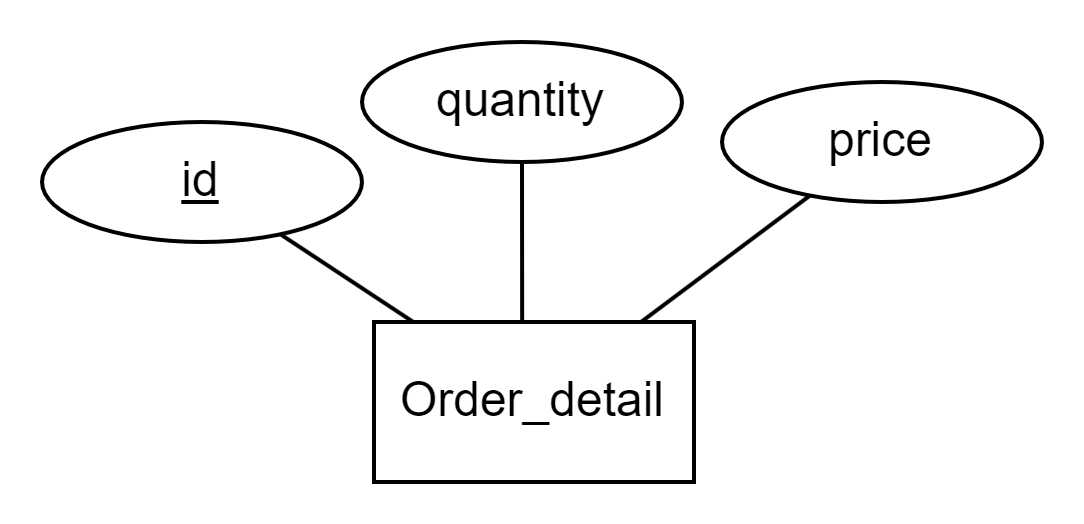
\includegraphics[width=11cm]{Images/ERD/order_detail.png}
            \newline
            \caption{Chi tiết thiết kế của thực thể Order detail}
            \label{fig:enter-label}
\end{figure}
Các thuộc tính của thực thể Order detail:
\begin{itemize}
\item id: Khóa chính, dùng để định danh cho mỗi variant có trong order
\item quantity: Số lượng của variant đó trong đơn hàng
\item price: Giá trị của toàn bộ variant đó trong đơn hàng
\end{itemize}

\begin{figure}[H]
            \centering
            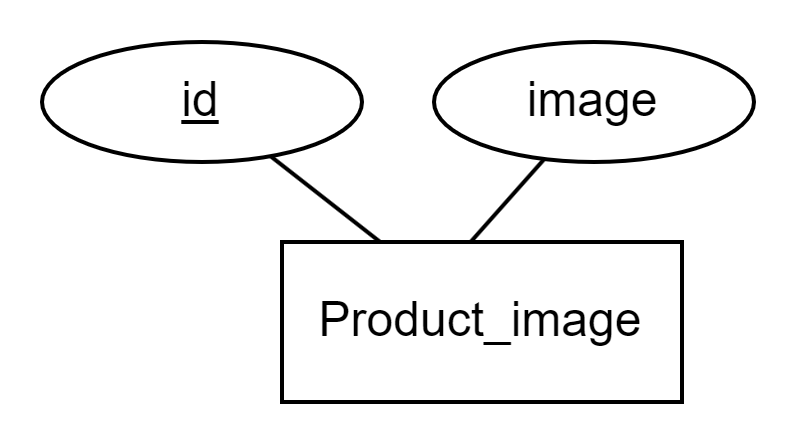
\includegraphics[width=11cm]{Images/ERD/product_image.png}
            \newline
            \caption{Chi tiết thiết kế của thực thể Product image}
            \label{fig:enter-label}
\end{figure}
Các thuộc tính của thực thể Order detail:
\begin{itemize}
\item id: Khóa chính, dùng để định danh cho mỗi ảnh
\item image: Đường dẫn(link) của ảnh đó
\end{itemize}

\newpage
\subsubsection{Thiết kế cơ sở dữ liệu vật lý}
Bảng Staff lưu trữ thông tin của các nhân viên
\begin{table}[H]
\centering
\begin{tabular}{|p{4cm}|p{3cm}|p{7cm}|}
\hline
Thuộc tính & Kiểu dữ liệu & Mô tả \\
\hline
id & integer & Khóa chính \\
\hline
name & varchar &  \\
\hline
email & varchar & \\
\hline
password & varchar & \\
\hline
phone\_number & varchar & \\
\hline
image & varchar & \\
\hline
password\_change\_at & timestamp & \\
\hline
last\_login\_at & timestamp &  \\
\hline
registry\_at & timestamp &  \\
\hline
role & varchar &  \\
\hline
\end{tabular}
\caption{Bảng thiết kế vật lý cho Staff}
\end{table}

\noindent Bảng Product\_image lưu trữ ảnh của sản phẩm
\begin{table}[H]
\centering
\begin{tabular}{|p{4cm}|p{3cm}|p{7cm}|}
\hline
Thuộc tính & Kiểu dữ liệu & Mô tả \\
\hline
id & integer & Khóa chính \\
\hline
color\_id & integer & Khóa ngoài tham chiếu tới color.id \\
\hline
image & varchar &  \\
\hline
product\_id & integer & Khóa ngoài tham chiếu tới product.id \\
\hline

\end{tabular}
\caption{Bảng thiết kế vật lý cho Product\_image}
\end{table}

\newpage
\noindent Bảng User lưu trữ thông tin người dùng
\begin{table}[H]
\centering
\begin{tabular}{|p{4cm}|p{3cm}|p{7cm}|}
\hline
Thuộc tính & Kiểu dữ liệu & Mô tả \\
\hline
id & integer & Khóa chính \\
\hline
name & varchar &  \\
\hline
email & varchar &  \\
\hline
password & varchar &  \\
\hline
phone\_number & varchar &  \\
\hline
image & varchar &  \\
\hline
password\_change\_at & timestamp &  \\
\hline
sex & varchar &  \\
\hline
date\_of\_birth & timestamp &  \\
\hline
last\_login\_at & timestamp &  \\
\hline
registry\_at & timestamp &  \\
\hline
otp\_code & varchar &  \\
\hline
otp\_expired\_at & timestamp &  \\
\hline

\end{tabular}
\caption{Bảng thiết kế vật lý cho User}
\end{table}

\noindent Bảng Color lưu trữ thông tin của màu
\begin{table}[H]
\centering
\begin{tabular}{|p{4cm}|p{3cm}|p{7cm}|}
\hline
Thuộc tính & Kiểu dữ liệu & Mô tả \\
\hline
id & integer & Khóa chính \\
\hline
name & varchar & \\
\hline
color\_code & varchar &  \\
\hline

\end{tabular}
\caption{Bảng thiết kế vật lý cho Color}
\end{table}

\newpage
\noindent Bảng Recipient\_information lưu thông tin của chi nhận hàng chi tiết của người dùng
\begin{table}[H]
\centering
\begin{tabular}{|p{4cm}|p{3cm}|p{7cm}|}
\hline
Thuộc tính & Kiểu dữ liệu & Mô tả \\
\hline
id & integer & Khóa chính \\
\hline
name & varchar &  \\
\hline
address & varchar &  \\
\hline
phone\_number & varchar &  \\
\hline
user\_id & integer &  Khóa ngoại tham khảo tới user.id\\
\hline
default\_recipient & boolean &  \\
\hline

\end{tabular}
\caption{Bảng thiết kế vật lý cho Recipient\_information}
\end{table}

\noindent Bảng Voucher lưu thông tin của voucher
\begin{table}[H]
\centering
\begin{tabular}{|p{4cm}|p{3cm}|p{7cm}|}
\hline
Thuộc tính & Kiểu dữ liệu & Mô tả \\
\hline
id & integer & Khóa chính \\
\hline
name & varchar & \\
\hline
create\_at & timestamp & \\
\hline
started\_at & timestamp & \\
\hline
expired\_at & timestamp & \\
\hline
max\_price & integer & \\
\hline
min\_price\_apply & integer & \\
\hline
percent\_discount & integer & \\
\hline
remaining\_quantity & integer & \\
\hline
type & varchar & \\
\hline
used\_quantity & integer & \\
\hline


\end{tabular}
\caption{Bảng thiết kế vật lý cho Voucher}
\end{table}
\newpage
\noindent Bảng User\_own\_voucher lưu thông tin người dùng nào sở hữu voucher
\begin{table}[H]
\centering
\begin{tabular}{|p{4cm}|p{3cm}|p{7cm}|}
\hline
Thuộc tính & Kiểu dữ liệu & Mô tả \\
\hline
id & integer & Khóa chính \\
\hline
user\_id & integer & Khóa ngoài tham chiếu tới user.id \\
\hline
voucher\_id & integer & Khóa ngoài tham chiếu tới voucher.id \\
\hline
status & boolean & \\
\hline

\end{tabular}
\caption{Bảng thiết kế vật lý cho User\_own\_voucher}
\end{table}

\noindent Bảng Category lưu thông tin các danh mục
\begin{table}[H]
\centering
\begin{tabular}{|p{4cm}|p{3cm}|p{7cm}|}
\hline
Thuộc tính & Kiểu dữ liệu & Mô tả \\
\hline
id & integer & Khóa chính \\
\hline
name & varchar & \\
\hline
image & varchar & \\
\hline
parent\_category\_id & integer & Khoá ngoại tham chiếu tới category.id\\
\hline

\end{tabular}
\caption{Bảng thiết kế vật lý cho Category}
\end{table}

\noindent Bảng Shipping\_method lưu thông tin phương thức vận chuyển
\begin{table}[H]
\centering
\begin{tabular}{|p{4cm}|p{3cm}|p{7cm}|}
\hline
Thuộc tính & Kiểu dữ liệu & Mô tả \\
\hline
id & integer & Khóa chính \\
\hline
name & varchar & \\
\hline
price & integer &\\
\hline

\end{tabular}
\caption{Bảng thiết kế vật lý cho Shipping\_method}
\end{table}

\noindent Bảng Payment\_method lưu thông tin phương thức thanh toán
\begin{table}[H]
\centering
\begin{tabular}{|p{4cm}|p{3cm}|p{7cm}|}
\hline
Thuộc tính & Kiểu dữ liệu & Mô tả \\
\hline
id & integer & Khóa chính \\
\hline
name & varchar & \\
\hline

\end{tabular}
\caption{Bảng thiết kế vật lý cho Payment\_method}
\end{table}

\newpage
\noindent Bảng Product lưu thông tin sản phẩm
\begin{table}[H]
\centering
\begin{tabular}{|p{4cm}|p{3cm}|p{7cm}|}
\hline
Thuộc tính & Kiểu dữ liệu & Mô tả \\
\hline
id & integer & Khóa chính \\
\hline
name & varchar &  \\
\hline
manufacturer & varchar &  \\
\hline
pattern & varchar &  \\
\hline
style & varchar &  \\
\hline
material & varchar &  \\
\hline
others & json &  \\
\hline
created\_at & timestamp &  \\
\hline
category\_id & integer &  \\
\hline
avg\_rating & float &  \\
\hline
\end{tabular}
\caption{Bảng thiết kế vật lý cho Product}
\end{table}


\noindent Bảng Variant lưu thông tin các biến thể của cùng một sản phẩm(product)

\begin{table}[H]
\centering
\begin{tabular}{|p{4cm}|p{3cm}|p{7cm}|}
\hline
Thuộc tính & Kiểu dữ liệu & Mô tả \\
\hline
id & integer & Khóa chính \\
\hline
size & varchar & \\
\hline
price\_import & integer & \\
\hline  
price\_sale & integer & \\
\hline
price\_export & integer & \\
\hline
percent\_sale & float & \\
\hline
remain\_quantity & integer & \\
\hline
update\_at & timestamp & \\
\hline
product\_id & intger & Khóa ngoại tham chiếu tới product.id \\
\hline
color\_id & integer &  Khóa ngoại tham chiếu tới color.id \\
\hline

\end{tabular}
\caption{Bảng thiết kế vật lý cho Variant}
\end{table}

\newpage


\noindent Bảng Order lưu thông tin của các đơn hàng
\begin{table}[H]
\centering
\begin{tabular}{|p{5cm}|p{2cm}|p{7cm}|}
\hline
Thuộc tính & Kiểu dữ liệu & Mô tả \\
\hline
id & integer & Khóa chính \\
\hline
state & varchar & \\
\hline
description & varchar & \\
\hline
amount & float & \\
\hline
created\_at & timestamp & \\
\hline
transaction\_at & timestamp & \\
\hline
confirm\_at & timestamp & \\
\hline
ship\_at & timestamp & \\
\hline
done\_at & timestamp & \\
\hline
cancel\_at & timestamp & \\
\hline
webhook\_data & json & \\
\hline
payment\_link & json & \\
\hline
recipient\_information\_id & integer & Khóa ngoại tham chiếu tới recipient\_information.id \\
\hline
shipping\_method\_id & integer & Khóa ngoại tham chiếu tới shipping\_method.id \\
\hline
payment\_method\_id & integer & Khóa ngoại tham chiếu tới payment\_method.id \\
\hline
voucher\_id & integer & Khóa ngoại tham chiếu tới voucher.id \\
\hline
\end{tabular}
\caption{Bảng thiết kế vật lý cho Order}
\end{table}

\noindent Bảng Variant\_apply\_voucher lưu thông tin các variant được áp dụng voucher
\begin{table}[H]
\centering
\begin{tabular}{|p{4cm}|p{3cm}|p{7cm}|}
\hline
Thuộc tính & Kiểu dữ liệu & Mô tả \\
\hline
id & integer & Khóa chính \\
\hline
voucher\_id & integer & Khóa ngoại tham chiếu tới voucher.id \\
\hline
variant\_id & integer & Khóa ngoại tham chiếu tới variant.id\\
\hline
\end{tabular}
\caption{Bảng thiết kế vật lý cho Variant\_apply\_voucher}
\end{table}

\newpage
\noindent Bảng Order\_detail lưu thông tin chi tiết từng sản phẩm thuộc đơn hàng

\begin{table}[H]
\centering
\begin{tabular}{|p{4cm}|p{3cm}|p{7cm}|}
\hline
Thuộc tính & Kiểu dữ liệu & Mô tả \\
\hline
id & integer & Khóa chính \\
\hline
quantity & integer & \\
\hline
price & integer & \\
\hline
variant\_id & integer & Khóa ngoại tham chiếu tới variant.id \\
\hline
order\_id & integer & Khóa ngoại tham chiếu tới order.id \\
\hline
\end{tabular}
\caption{Bảng thiết kế vật lý cho Order\_detail}
\end{table}


\noindent Bảng Review lưu thông tin nhận xét sản phẩm của mỗi lần đặt hàng của người dùng

\begin{table}[H]
\centering
\begin{tabular}{|p{4cm}|p{3cm}|p{7cm}|}
\hline
Thuộc tính & Kiểu dữ liệu & Mô tả \\
\hline
id & integer & Khóa chính \\
\hline
rating & integer & \\
\hline
image & varchar & \\
\hline
content & varchar & \\
\hline
created\_at & timestamp & \\
\hline
user\_id & integer & Khóa ngoại tham chiếu tới user.id \\
\hline
order\_detail\_id & integer & Khóa ngoại tham chiếu tới order\_detail.id \\
\hline
is\_disable & boolean & \\
\hline

\end{tabular}
\caption{Bảng thiết kế vật lý cho Review}
\end{table}

\newpage
\noindent Bảng Analyze\_product\_monthly lưu thông tin doanh số bán của một sản phẩm trong từng tháng
\begin{table}[H]
\centering
\begin{tabular}{|p{4cm}|p{3cm}|p{7cm}|}
\hline
Thuộc tính & Kiểu dữ liệu & Mô tả \\
\hline
id & integer & Khóa chính \\
\hline
year & integer & \\
\hline
month & integer & \\
\hline
quantity & integer & \\
\hline
product\_id & integer & Khóa ngoại tham chiếu tới product.id \\
\hline

\end{tabular}
\caption{Bảng thiết kế vật lý cho Analyze\_product\_monthly}
\end{table}

\noindent Bảng Category\_apply\_voucher lưu thông tin các thể loại/danh mục được áp dụng voucher
\begin{table}[H]
\centering
\begin{tabular}{|p{4cm}|p{3cm}|p{7cm}|}
\hline
Thuộc tính & Kiểu dữ liệu & Mô tả \\
\hline
id & integer & Khóa chính \\
\hline
voucher\_id & integer & Khóa ngoại tham chiếu tới voucher.id \\
\hline
category\_id & integer & Khóa ngoại tham chiếu tới category.id\\
\hline
\end{tabular}
\caption{Bảng thiết kế vật lý cho Category\_apply\_voucher}
\end{table}

\noindent Bảng Product\_apply\_voucher lưu thông tin các sản phẩm được áp dụng voucher
\begin{table}[H]
\centering
\begin{tabular}{|p{4cm}|p{3cm}|p{7cm}|}
\hline
Thuộc tính & Kiểu dữ liệu & Mô tả \\
\hline
id & integer & Khóa chính \\
\hline
voucher\_id & integer & Khóa ngoại tham chiếu tới voucher.id \\
\hline
product\_id & integer & Khóa ngoại tham chiếu tới product.id\\
\hline
\end{tabular}
\caption{Bảng thiết kế vật lý cho Product\_apply\_voucher}
\end{table}



   
